\documentclass[12pt,a4paper]{article}

% ------------------------------------------------------------------
% Ngôn ngữ và font
% ------------------------------------------------------------------
\usepackage{fontspec}
\usepackage{polyglossia}
\setdefaultlanguage{vietnamese}
\setmainfont{DejaVu Serif}
\setsansfont{DejaVu Sans}
\setmonofont{Liberation Mono}[Scale=0.86]

\usepackage[a4paper,top=2.2cm,bottom=2.2cm,left=2.5cm,right=2.2cm,headheight=14pt]{geometry}
\usepackage{graphicx}
\usepackage{float}
\usepackage{booktabs}
\usepackage{tabularx}
\usepackage{array}
\usepackage{multirow}
\usepackage{makecell}
\usepackage[table]{xcolor}
\usepackage{tikz}
\usetikzlibrary{positioning,arrows.meta,calc,fit,backgrounds,shapes.geometric}
\usepackage{listings}
\usepackage{caption}
\usepackage{enumitem}
\usepackage{fancyhdr}
\usepackage{titlesec}
\usepackage{tocloft}
\usepackage[hidelinks,unicode=true,pdfencoding=auto]{hyperref}
\hypersetup{
  pdftitle={Báo cáo PBL3: Định tuyến động RIPv2 và máy chủ DHCP trên GNS3},
  pdfauthor={Thái Viết Đại, Phan Văn Trà},
  pdfsubject={Tái triển khai bài lab RIPv2 và DHCP trên GNS3 với FRRouting và Docker}
}

% ------------------------------------------------------------------
% Màu và định dạng chung
% ------------------------------------------------------------------
\definecolor{primary}{HTML}{000000}
\definecolor{accent}{HTML}{000000}
\definecolor{passgreen}{HTML}{1A7F37}
\definecolor{codebg}{HTML}{F6F8FA}
\definecolor{codeborder}{HTML}{D0D7DE}
\definecolor{rulegray}{HTML}{BFC7D1}

\setlength{\parindent}{1.15em}
\setlength{\parskip}{0.32em}
\setlength{\emergencystretch}{3em}
\linespread{1.12}
\renewcommand{\arraystretch}{1.16}

\captionsetup{font=small,labelfont=bf,labelsep=period,justification=centering,skip=6pt}
\renewcommand{\lstlistingname}{Đoạn mã}

\titleformat{\section}[block]{\sffamily\Large\bfseries\color{primary}}{\thesection.}{0.55em}{}
\titlespacing*{\section}{0pt}{14pt}{6pt}
\titleformat{\subsection}[block]{\sffamily\large\bfseries\color{black}}{\thesubsection}{0.55em}{}
\titlespacing*{\subsection}{0pt}{10pt}{4pt}
\titleformat{\subsubsection}[block]{\sffamily\normalsize\bfseries\color{accent}}{\thesubsubsection}{0.55em}{}

\renewcommand{\thesection}{\Roman{section}}
\renewcommand{\thesubsection}{\arabic{section}.\arabic{subsection}}
\renewcommand{\thesubsubsection}{\thesubsection.\arabic{subsubsection}}
\renewcommand{\contentsname}{MỤC LỤC}

% Thu gọn mục lục và đủ chỗ cho số thứ tự La Mã
\setlength{\cftbeforetoctitleskip}{0pt}
\setlength{\cftaftertoctitleskip}{8pt}
\renewcommand{\cfttoctitlefont}{\sffamily\Large\bfseries\color{primary}}
\setlength{\cftsecindent}{0em}
\setlength{\cftsecnumwidth}{3.2em}
\setlength{\cftsubsecindent}{2.2em}
\setlength{\cftsubsecnumwidth}{4.2em}
\setlength{\cftsubsubsecindent}{4.4em}
\setlength{\cftsubsubsecnumwidth}{5.2em}
\setlength{\cftbeforesecskip}{2pt}
\setlength{\cftbeforesubsecskip}{0pt}
\setlength{\cftbeforesubsubsecskip}{0pt}
\renewcommand{\figurename}{Hình}
\renewcommand{\tablename}{Bảng}

\pagestyle{fancy}
\fancyhf{}
\fancyhead[L]{\small\sffamily\color{primary}PBL3 -- RIPv2 \& DHCP trên GNS3}
\fancyhead[R]{\small\sffamily\color{primary}Trang \thepage}
\renewcommand{\headrulewidth}{0.4pt}

% ------------------------------------------------------------------
% Listing style
% ------------------------------------------------------------------
\lstdefinelanguage{FRR}{
  morekeywords={hostname,interface,ip,address,no,shutdown,exit,router,rip,version,network,log,syslog,debug,ipv6,route},
  morecomment=[l]{!},
  sensitive=true
}

\lstdefinestyle{frr}{
  language=FRR,
  basicstyle=\ttfamily\footnotesize,
  keywordstyle=\color{primary}\bfseries,
  commentstyle=\color{black}\itshape,
  backgroundcolor=\color{codebg},
  frame=single,
  rulecolor=\color{codeborder},
  framerule=0.4pt,
  numbers=left,
  numberstyle=\tiny\color{black},
  numbersep=8pt,
  breaklines=true,
  postbreak=\mbox{\textcolor{black}{$\hookrightarrow$}\space},
  showstringspaces=false,
  columns=fullflexible,
  keepspaces=true,
  xleftmargin=1.8em,
  framexleftmargin=1.4em,
  aboveskip=8pt,
  belowskip=6pt
}

\lstdefinestyle{plaincode}{
  basicstyle=\ttfamily\footnotesize,
  backgroundcolor=\color{codebg},
  frame=single,
  rulecolor=\color{codeborder},
  framerule=0.4pt,
  numbers=left,
  numberstyle=\tiny\color{black},
  numbersep=8pt,
  breaklines=true,
  showstringspaces=false,
  columns=fullflexible,
  keepspaces=true,
  xleftmargin=1.8em,
  framexleftmargin=1.4em,
  aboveskip=8pt,
  belowskip=6pt
}

% ------------------------------------------------------------------
% Kiểu node cho sơ đồ TikZ
% ------------------------------------------------------------------
\tikzset{
  router/.style={draw=primary,fill=primary!10,rounded corners=4pt,
    minimum width=2.1cm,minimum height=0.95cm,align=center,
    font=\sffamily\bfseries\small},
  switch/.style={draw=teal!70!black,fill=teal!10,rounded corners=3pt,
    minimum width=1.9cm,minimum height=0.8cm,align=center,
    font=\sffamily\bfseries\scriptsize},
  pc/.style={draw=black!55,fill=black!6,rounded corners=3pt,
    minimum width=1.55cm,minimum height=0.7cm,align=center,
    font=\sffamily\scriptsize},
  server/.style={draw=orange!80!black,fill=orange!12,rounded corners=3pt,
    minimum width=2.0cm,minimum height=0.85cm,align=center,
    font=\sffamily\bfseries\scriptsize},
  wan/.style={line width=1.3pt,draw=primary!85!black},
  lan/.style={line width=0.9pt,draw=teal!65!black},
  edge/.style={line width=0.7pt,draw=black!55}
}

\begin{document}
\pagenumbering{roman}

% ==================================================================
% TRANG BÌA
% ==================================================================
\begin{titlepage}
  \thispagestyle{empty}
  \centering
  \vspace*{1.1cm}

  {\sffamily\large\color{primary} BÁO CÁO BÀI TẬP LỚN (PBL3)\par}
  \vspace{0.35cm}
  {\color{primary}\rule{0.82\textwidth}{1.2pt}\par}
  \vspace{1.3cm}

  {\sffamily\bfseries\fontsize{27}{33}\selectfont
    ĐỊNH TUYẾN ĐỘNG RIPv2\\[0.25cm]
    VÀ MÁY CHỦ DHCP\par}

  \vspace{0.9cm}
  {\sffamily\Large\color{primary}
    TRIỂN KHAI TRÊN GNS3\\[0.15cm]
    VỚI FRROUTING VÀ DOCKER\par}

  \vspace{0.45cm}
  {\color{primary}\rule{0.55\textwidth}{0.6pt}\par}

  \vspace{2.0cm}
  {\sffamily\normalsize
    \renewcommand{\arraystretch}{1.45}
    \begin{tabular}{@{}l@{\hspace{0.45cm}}l@{}}
      Người thực hiện:& \textbf{Thái Viết Đại} \\
                      & \textbf{Phan Văn Trà} \\
      Giảng viên hướng dẫn: & \textbf{TS. Đào Duy Tuấn} \\
      Hình thức:      & Báo cáo thực hành mạng máy tính \\
      Môi trường:     & GNS3 3.0.6, FRRouting 8.4, \\
                      & Docker, VPCS 0.8.5 \\
    \end{tabular}\par}

  \vfill
  {\sffamily\small\color{black}
    Báo cáo được xây dựng dựa trên đề bài và bố cục của báo cáo PBL3 gốc\\
    trên Cisco Packet Tracer, sau đó tái triển khai và kiểm thử trên GNS3.\par}
  \vspace{0.4cm}
  {\sffamily\small Tháng 10 năm 2026\par}
\end{titlepage}
\pagenumbering{arabic}

% ==================================================================
% TÓM TẮT
% ==================================================================
\newpage
\section*{Tóm tắt}
\addcontentsline{toc}{section}{Tóm tắt}

Báo cáo trình bày quá trình tái triển khai bài lab PBL3 ``Định tuyến động RIPv2 và máy chủ DHCP''
trên nền tảng \textbf{GNS3 3.0.6}. Thiết kế mạng giữ nguyên theo báo cáo gốc: bốn router R0--R3
kết nối thành vòng, bốn mạng LAN ``A'', ``B'', ``C'', ``D'' tương ứng với bốn switch, và một DHCP
server đặt tại Network A. Thay vì dùng Cisco IOSv cần image có bản quyền, các router được triển khai
bằng \textbf{FRRouting 8.4} chạy trong container Docker; DHCP server dùng Alpine Linux với BusyBox
\texttt{udhcpd}; các máy trạm dùng VPCS 0.8.5.

Toàn bộ topology, địa chỉ IP và cấu hình được tạo tự động qua GNS3 API v3 bằng Python. Sau khi
RIPv2 hội tụ, cả bốn router đều học đủ ba mạng LAN còn lại; PC\_A nhận địa chỉ động trong dải
\texttt{192.168.10.10--192.168.10.100}; các phép ping liên mạng từ PC\_A và PC\_D đều thành công.
Bộ kiểm thử tự động \texttt{test.sh} ghi nhận \textbf{9/9} hạng mục PASS. Báo cáo cũng phân tích
các vấn đề kỹ thuật gặp phải khi chuyển từ Packet Tracer sang GNS3/FRR.

\newpage
\tableofcontents
\newpage

% ==================================================================
\section{TỔNG QUAN ĐỀ BÀI VÀ MỤC TIÊU}
% ==================================================================

\subsection{Đề bài}

Thiết lập mô hình mạng gồm bốn router R0, R1, R2, R3 kết nối với nhau theo dạng vòng
(ring topology). Trên tất cả router, cấu hình giao thức định tuyến động RIPv2 để bảo đảm
liên thông toàn mạng. Tại Network A, triển khai một DHCP server để tự động cấp phát địa chỉ
IP cho các máy trạm kết nối vào switch của mạng này. Bốn mạng LAN được đánh số như sau:

\begin{itemize}[leftmargin=1.6em,itemsep=2pt]
  \item Network A: \texttt{192.168.10.0/24}, gateway \texttt{192.168.10.1} (R0).
  \item Network B: \texttt{192.168.20.0/24}, gateway \texttt{192.168.20.1} (R1).
  \item Network C: \texttt{192.168.30.0/24}, gateway \texttt{192.168.30.1} (R2).
  \item Network D: \texttt{192.168.40.0/24}, gateway \texttt{192.168.40.1} (R3).
\end{itemize}

\subsection{Mục tiêu bài lab}

\begin{enumerate}[leftmargin=1.7em,itemsep=2pt]
  \item Thiết lập đúng sơ đồ kết nối vật lý và logic cho bốn router cùng bốn mạng LAN.
  \item Gán địa chỉ IP chính xác cho tất cả interface của router, DHCP server và máy trạm.
  \item Triển khai RIPv2 trên toàn bộ router, kiểm tra bảng định tuyến và trạng thái tiến trình RIP.
  \item Triển khai DHCP server tại Network A, cấp phát động địa chỉ trong dải
        \texttt{192.168.10.10--192.168.10.100} với gateway và DNS là \texttt{192.168.10.1}.
  \item Kiểm tra khả năng liên thông end-to-end bằng ping từ Network A sang gateway của các mạng
        còn lại và theo chiều ngược lại.
  \item Tự động hóa việc tạo topology, cấu hình và kiểm thử bằng Python thông qua GNS3 API.
\end{enumerate}

\subsection{Phạm vi và lựa chọn triển khai}

Báo cáo gốc thực hiện bài lab trên Cisco Packet Tracer với router mô phỏng của Packet Tracer và
DHCP server dạng Server0. Báo cáo này giữ nguyên thiết kế về topology, địa chỉ IP, vai trò các
node và kịch bản kiểm thử, nhưng thay đổi nền tảng triển khai:

\begin{itemize}[leftmargin=1.6em,itemsep=2pt]
  \item \textbf{GNS3 3.0.6} thay cho Packet Tracer: GNS3 cho phép chạy các node mạng thật
        (Docker, máy ảo, thiết bị phần cứng) và quản lý qua API.
  \item \textbf{FRRouting 8.4} trong Docker thay cho Cisco IOS: FRR là bộ định tuyến mã nguồn mở,
        hỗ trợ RIPv2 thật và có CLI \texttt{vtysh} gần với thao tác của IOS. Cách này không cần
        image Cisco IOSv có bản quyền.
  \item \textbf{Alpine Linux + BusyBox \texttt{udhcpd}} thay cho Server0 của Packet Tracer.
  \item \textbf{VPCS 0.8.5} thay cho các Laptop mô phỏng, hỗ trợ cả DHCP và IP tĩnh.
\end{itemize}

Việc thay thế chỉ tác động đến công cụ mô phỏng, không làm thay đổi logic của bài lab. Đây cũng
là nội dung chính được trình bày trong các chương sau.

% ==================================================================
\section{SƠ ĐỒ MẠNG VÀ BẢNG PHÂN BỔ ĐỊA CHỈ IP}
% ==================================================================

\subsection{Sơ đồ mạng theo báo cáo gốc}

Hình~\ref{fig:original} là sơ đồ mạng vòng bốn router được trích từ báo cáo PBL3 gốc. Sơ đồ thể
hiện bốn router R0--R3 nối thành vòng, mỗi router quản lý một mạng LAN thông qua switch, và
DHCP server nằm trong Network A.

\begin{figure}[H]
  \centering
  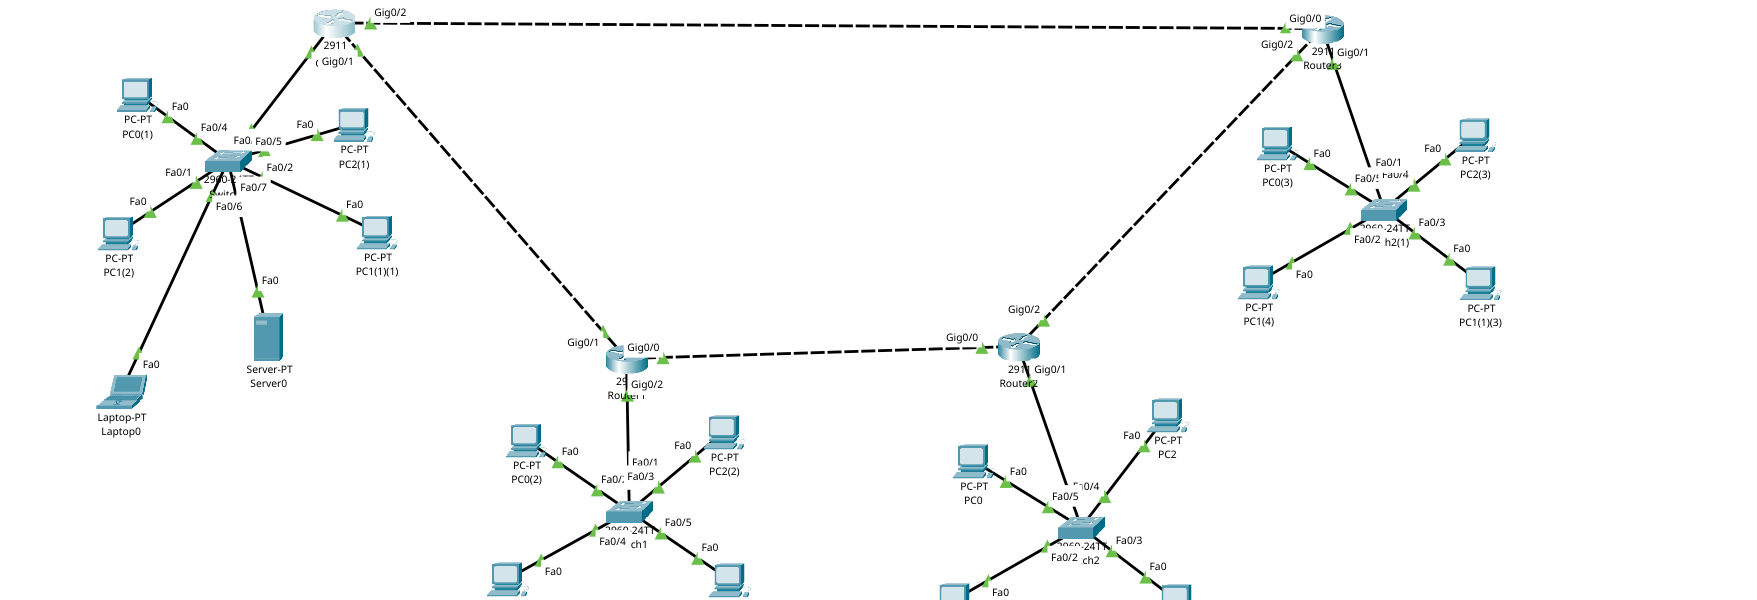
\includegraphics[width=\textwidth]{images/original-topology.png}
  \caption{Sơ đồ mạng vòng bốn router trong báo cáo gốc (Packet Tracer).}
  \label{fig:original}
\end{figure}

\subsection{Sơ đồ triển khai trên GNS3}

Hình~\ref{fig:topology} là sơ đồ triển khai thực tế trên GNS3. Bốn router FRR được đặt tại bốn
đỉnh của vòng; mỗi router nối tới một switch LAN, từ switch nối tới máy trạm. DHCP server nối
vào \texttt{SW\_A} và có địa chỉ \texttt{192.168.10.2}. Các đường nét đậm là liên kết WAN giữa
các router; các đường nét mảnh là liên kết LAN.

\begin{figure}[H]
  \centering
  \resizebox{\textwidth}{!}{%
  \begin{tikzpicture}
    % --- Router ---
    \node[router] (R0) at (-3.8,0)   {R0};
    \node[router] (R1) at (0,2.8)    {R1};
    \node[router] (R2) at (3.8,0)    {R2};
    \node[router] (R3) at (0,-2.8)   {R3};

    % --- Switch LAN ---
    \node[switch] (SWA) at (-6.2,0)  {SW\_A};
    \node[switch] (SWB) at (0,5.0)   {SW\_B};
    \node[switch] (SWC) at (6.2,0)   {SW\_C};
    \node[switch] (SWD) at (0,-5.0)  {SW\_D};

    % --- Client / server ---
    \node[pc]     (PCA)  at (-8.2,-1.0) {PC\_A};
    \node[server] (DHCP) at (-8.2,1.0)  {DHCP\\Server};
    \node[pc]     (PCB)  at (1.9,5.0)   {PC\_B};
    \node[pc]     (PCC)  at (8.2,1.0)   {PC\_C};
    \node[pc]     (PCD)  at (-1.9,-5.0) {PC\_D};

    % --- WAN ring ---
    \draw[wan] (R0) -- node[above,sloped,font=\scriptsize,fill=white,inner sep=1pt]
      {10.0.12.0/30} (R1);
    \draw[wan] (R1) -- node[above,sloped,font=\scriptsize,fill=white,inner sep=1pt]
      {10.0.23.0/24} (R2);
    \draw[wan] (R2) -- node[above,sloped,font=\scriptsize,fill=white,inner sep=1pt]
      {10.0.34.0/24} (R3);
    \draw[wan] (R3) -- node[above,sloped,font=\scriptsize,fill=white,inner sep=1pt]
      {10.0.41.0/24} (R0);

    % --- LAN links ---
    \draw[lan] (R0) -- node[above=10pt,align=center,font=\scriptsize,fill=white,inner sep=1pt]
      {LAN A\\192.168.10.0/24} (SWA);
    \draw[lan] (R1) -- node[right,align=left,font=\scriptsize,fill=white,inner sep=1pt]
      {LAN B\\192.168.20.0/24} (SWB);
    \draw[lan] (R2) -- node[above=10pt,align=center,font=\scriptsize,fill=white,inner sep=1pt]
      {LAN C\\192.168.30.0/24} (SWC);
    \draw[lan] (R3) -- node[right,align=left,font=\scriptsize,fill=white,inner sep=1pt]
      {LAN D\\192.168.40.0/24} (SWD);

    % --- Access links ---
    \draw[edge] (SWA) -- (PCA);
    \draw[edge] (SWA) -- (DHCP);
    \draw[edge] (SWB) -- (PCB);
    \draw[edge] (SWC) -- (PCC);
    \draw[edge] (SWD) -- (PCD);

    \node[below=3pt of DHCP,font=\scriptsize,text=black]
      {pool .10--.100};
    \node[above=1pt of PCB,font=\scriptsize,text=black] {static .10};
    \node[above=1pt of PCC,font=\scriptsize,text=black] {static .10};
    \node[below=1pt of PCD,font=\scriptsize,text=black] {static .10};
  \end{tikzpicture}}
  \caption{Sơ đồ triển khai trên GNS3: router FRR, switch LAN, PC và DHCP server.}
  \label{fig:topology}
\end{figure}

\subsection{Bảng liên kết WAN}

Bảng~\ref{tab:wan} tóm tắt bốn liên kết WAN tạo thành vòng. Liên kết R0--R1 dùng subnet
\texttt{/30} theo đúng báo cáo gốc; ba liên kết còn lại dùng \texttt{/24}.

\begin{table}[H]
  \centering
  \caption{Các liên kết WAN trong mô hình.}
  \label{tab:wan}
  \begin{tabularx}{\textwidth}{@{}l l l X@{}}
    \toprule
    \textbf{Kết nối} & \textbf{Mạng WAN} & \textbf{Subnet mask} & \textbf{Ghi chú} \\
    \midrule
    R0 -- R1 & 10.0.12.0/30 & 255.255.255.252 & Liên kết trực tiếp, subnet nhỏ nhất \\
    R1 -- R2 & 10.0.23.0/24 & 255.255.255.0   & Liên kết trực tiếp \\
    R2 -- R3 & 10.0.34.0/24 & 255.255.255.0   & Liên kết trực tiếp \\
    R3 -- R0 & 10.0.41.0/24 & 255.255.255.0   & Liên kết trực tiếp \\
    \bottomrule
  \end{tabularx}
\end{table}

\subsection{Bảng phân bổ địa chỉ IP}

Bảng~\ref{tab:ip} liệt kê địa chỉ IP trên từng interface. Tên interface được giữ theo cách đặt
của FRR trong container (\texttt{eth0}, \texttt{eth1}, \texttt{eth2}); vai trò và thứ tự kết nối
tương ứng với các cổng GigabitEthernet trong báo cáo gốc.

\begin{table}[H]
  \centering
  \caption{Bảng phân bổ địa chỉ IP.}
  \label{tab:ip}
  \small
  \begin{tabularx}{\textwidth}{@{}l l l l X@{}}
    \toprule
    \textbf{Thiết bị} & \textbf{Interface} & \textbf{Địa chỉ IP} & \textbf{Subnet mask} & \textbf{Kết nối / ghi chú} \\
    \midrule
    \multirow{3}{*}{R0}
      & eth0 & 192.168.10.1 & 255.255.255.0   & Gateway Network A (SW\_A) \\
      & eth1 & 10.0.12.1    & 255.255.255.252 & Kết nối R0 -- R1 \\
      & eth2 & 10.0.41.2    & 255.255.255.0   & Kết nối R0 -- R3 \\
    \midrule
    \multirow{3}{*}{R1}
      & eth0 & 10.0.23.1    & 255.255.255.0   & Kết nối R1 -- R2 \\
      & eth1 & 192.168.20.1 & 255.255.255.0   & Gateway Network B (SW\_B) \\
      & eth2 & 10.0.12.2    & 255.255.255.252 & Kết nối R1 -- R0 \\
    \midrule
    \multirow{3}{*}{R2}
      & eth0 & 10.0.23.2    & 255.255.255.0   & Kết nối R2 -- R1 \\
      & eth1 & 192.168.30.1 & 255.255.255.0   & Gateway Network C (SW\_C) \\
      & eth2 & 10.0.34.1    & 255.255.255.0   & Kết nối R2 -- R3 \\
    \midrule
    \multirow{3}{*}{R3}
      & eth0 & 10.0.41.1    & 255.255.255.0   & Kết nối R3 -- R0 \\
      & eth1 & 192.168.40.1 & 255.255.255.0   & Gateway Network D (SW\_D) \\
      & eth2 & 10.0.34.2    & 255.255.255.0   & Kết nối R3 -- R2 \\
    \midrule
    DHCP server & eth0 & 192.168.10.2 & 255.255.255.0 & Gateway: 192.168.10.1 \\
    \bottomrule
  \end{tabularx}
\end{table}

\subsection{Dải địa chỉ DHCP}

DHCP server chỉ phục vụ Network A. Cấu hình pool gồm: địa chỉ bắt đầu
\texttt{192.168.10.10}, địa chỉ kết thúc \texttt{192.168.10.100}, gateway mặc định
\texttt{192.168.10.1} và DNS \texttt{192.168.10.1}. Các máy PC\_B, PC\_C, PC\_D dùng địa chỉ
tĩnh lần lượt là \texttt{192.168.20.10}, \texttt{192.168.30.10}, \texttt{192.168.40.10} để bảo
đảm kết quả kiểm thử ổn định.

% ==================================================================
\section{CÔNG NGHỆ VÀ KIẾN TRÚC TRIỂN KHAI}
% ==================================================================

\subsection{GNS3 và API v3}

GNS3 3.0.6 được chạy ở chế độ local server tại \texttt{http://127.0.0.1:3080}, sử dụng API v3.
Mỗi project GNS3 là một tập hợp các node và link; các node Docker được GNS3 quản lý qua Docker
engine trên cùng máy. Trong bài lab, compute ``local'' cung cấp cả ba loại node cần thiết:
\texttt{docker}, \texttt{vpcs} và \texttt{ethernet\_switch}.

Các thao tác tạo project, node, link và cấu hình console đều được thực hiện bằng Python thay vì
thao tác thủ công trên GUI. Cách làm này bảo đảm lab có thể tái lập, đồng thời giảm sai sót khi
phải tạo 13 node và 13 liên kết.

\subsection{FRRouting trong Docker}

Mỗi router là một container từ image \texttt{frrouting/frr:latest}, chạy FRRouting 8.4. Bên trong
container, các tiến trình chính gồm \texttt{zebra} (quản lý interface và bảng định tuyến),
\texttt{ripd} (tiến trình RIPv2) và \texttt{staticd} (route tĩnh). Cấu hình được đưa vào container
qua \texttt{start\_command} của GNS3; sau khi khởi động, có thể kiểm tra bằng \texttt{vtysh}.

RIPv2 trong bài lab được cấu hình với \texttt{version 2}, quảng bá các mạng LAN và WAN bằng câu
lệnh \texttt{network}. RIPv2 là giao thức classless, gửi kèm subnet mask trong bản tin cập nhật;
FRR 8.4 không cung cấp lệnh \texttt{no auto-summary} như IOS, nhưng hành vi classless vẫn được
bảo đảm. Đây là điểm khác biệt cần lưu ý khi đối chiếu với báo cáo gốc.

Các thông số RIPv2 quan sát được trên R0: gửi cập nhật mỗi 30 giây (sai lệch $\pm 50\%$), timeout
sau 180 giây, garbage collect sau 120 giây, gửi và nhận version 2 trên cả ba interface, administrative
distance mặc định 120.

\subsection{DHCP server}

DHCP server là container Alpine Linux 3.20, chạy BusyBox \texttt{udhcpd} ở chế độ foreground.
Cấu hình được ghi vào \texttt{/etc/udhcpd.conf} với interface \texttt{eth0}, pool
\texttt{192.168.10.10--192.168.10.100}, gateway và DNS \texttt{192.168.10.1}. BusyBox
\texttt{udhcpd} là lựa chọn nhẹ, không cần cài thêm gói và phù hợp với môi trường container.

\subsection{Máy trạm VPCS}

Bốn máy trạm dùng VPCS 0.8.5. PC\_A được cấu hình \texttt{ip dhcp} để nhận địa chỉ động; PC\_B,
PC\_C, PC\_D được cấu hình IP tĩnh với gateway tương ứng. VPCS cung cấp các lệnh \texttt{show ip}
và \texttt{ping}, đủ để kiểm tra cấu hình và liên thông mà không cần hệ điều hành đầy đủ.

\subsection{Kiến trúc tự động hóa}

Bộ script Python gồm các thành phần sau:

\begin{table}[H]
  \centering
  \caption{Các script và vai trò trong bộ lab.}
  \label{tab:scripts}
  \begin{tabularx}{\textwidth}{@{}l X@{}}
    \toprule
    \textbf{File} & \textbf{Vai trò} \\
    \midrule
    \texttt{doctor.py} & Kiểm tra GNS3 API, template, compute, Docker image, VPCS, Dynamips,
      \texttt{ubridge} và BusyBox trước khi chạy lab. \\
    \texttt{setup.py} & Tạo project, template, 13 node, 13 link; gán IP và cấu hình RIPv2/DHCP;
      lưu \texttt{state.json}. \\
    \texttt{test.py} & Kiểm tra bảng định tuyến, trạng thái RIP, ping từ bốn PC và DHCP client;
      trả mã lỗi nếu có hạng mục FAIL. \\
    \texttt{cleanup.py} & Xóa project và template do lab tạo, có xác nhận trước khi xóa. \\
    \texttt{common.py} & Hàm dùng chung: gọi API, load/save state, đường dẫn log. \\
    \bottomrule
  \end{tabularx}
\end{table}

Quy trình chạy lab gồm bốn bước: \texttt{./doctor.sh} kiểm tra môi trường; \texttt{./setup.sh}
tạo topology và cấu hình; đợi khoảng 15 giây để RIPv2 và DHCP hội tụ; \texttt{./test.sh} kiểm thử
tự động. Kết quả và log được lưu trong thư mục \texttt{logs/} và \texttt{state.json}.

% ==================================================================
\section{NỘI DUNG CẤU HÌNH}
% ==================================================================

\subsection{Cấu hình FRR cho R0}

Đoạn mã~\ref{lst:r0} là cấu hình đầy đủ của R0. Cấu hình R1--R3 có cùng cấu trúc, chỉ khác địa
chỉ IP và các mạng được quảng bá; toàn bộ được trình bày trong Phụ lục~\ref{app:configs}.

\lstinputlisting[style=frr,caption={Cấu hình FRR của R0.},label={lst:r0}]
  {artifacts/configs/R0.conf}

\subsection{Tóm tắt cấu hình R1, R2, R3}

Bảng~\ref{tab:routers} tóm tắt interface và các mạng được quảng bá bởi ba router còn lại.

\begin{table}[H]
  \centering
  \caption{Interface và mạng quảng bá của R1--R3.}
  \label{tab:routers}
  \small
  \begin{tabularx}{\textwidth}{@{}l l l X@{}}
    \toprule
    \textbf{Router} & \textbf{LAN} & \textbf{Interface LAN} & \textbf{Mạng WAN và subnet} \\
    \midrule
    R1 & 192.168.20.0/24 & eth1: 192.168.20.1/24 &
      eth0: 10.0.23.1/24 (R1--R2); eth2: 10.0.12.2/30 (R1--R0) \\
    R2 & 192.168.30.0/24 & eth1: 192.168.30.1/24 &
      eth0: 10.0.23.2/24 (R2--R1); eth2: 10.0.34.1/24 (R2--R3) \\
    R3 & 192.168.40.0/24 & eth1: 192.168.40.1/24 &
      eth0: 10.0.41.1/24 (R3--R0); eth2: 10.0.34.2/24 (R3--R2) \\
    \bottomrule
  \end{tabularx}
\end{table}

\subsection{Cấu hình DHCP server}

Đoạn mã~\ref{lst:dhcp} là nội dung \texttt{/etc/udhcpd.conf} trong container DHCP. Server lắng
nghe trên \texttt{eth0}, cấp địa chỉ trong dải \texttt{.10--.100}, đồng thời cung cấp gateway và
DNS là \texttt{192.168.10.1}.

\lstinputlisting[style=plaincode,caption={Cấu hình BusyBox \texttt{udhcpd}.},label={lst:dhcp}]
  {artifacts/configs/udhcpd.conf}

\subsection{Cấu hình máy trạm VPCS}

PC\_A nhận cấu hình động; ba máy còn lại dùng IP tĩnh. Các lệnh tiêu biểu:

\begin{lstlisting}[style=plaincode,caption={Lệnh cấu hình và kiểm tra trên VPCS.},label={lst:vpcs}]
# PC_A
ip dhcp
show ip

# PC_B
ip 192.168.20.10/24 192.168.20.1
show ip

# PC_C
ip 192.168.30.10/24 192.168.30.1

# PC_D
ip 192.168.40.10/24 192.168.40.1
\end{lstlisting}

\subsection{Một số điểm kỹ thuật khi tự động hóa}

\begin{itemize}[leftmargin=1.6em,itemsep=2pt]
  \item \textbf{Gửi \texttt{start\_command} qua API v3:} trường này phải nằm trong
        \texttt{properties} của node Docker. Nếu gửi ở cấp ngoài cùng, GNS3 sẽ bỏ qua và container
        khởi động mà không có cấu hình.
  \item \textbf{Đặt tên container:} GNS3 tạo tên dạng
        \texttt{GNS3.<tên\_node>.<project\_id>}. Tên node \texttt{DHCP-Server} được giữ nguyên
        trong tên container; tên có dấu gạch dưới như \texttt{DHCP\_Server} được xử lý tương ứng.
  \item \textbf{Console VPCS:} sau khi kết nối lại, VPCS có thể chưa in prompt ngay. Script gửi
        một ký tự xuống dòng trước khi \texttt{expect} prompt để tránh treo.
  \item \textbf{Kiểm tra router FRR:} image FRR không chạy telnet console, nên dùng
        \texttt{docker exec <container> vtysh -c "show ip route"} thay cho console GNS3.
  \item \textbf{Lệnh RIP:} FRR dùng \texttt{show ip rip status}; lệnh
        \texttt{show ip protocols} của IOS không có trong FRR.
\end{itemize}

% ==================================================================
\section{KẾT QUẢ THỰC NGHIỆM}
% ==================================================================

\subsection{Môi trường thử nghiệm}

\begin{table}[H]
  \centering
  \caption{Môi trường chạy lab.}
  \label{tab:env}
  \begin{tabularx}{\textwidth}{@{}l l X@{}}
    \toprule
    \textbf{Thành phần} & \textbf{Phiên bản} & \textbf{Ghi chú} \\
    \midrule
    Hệ điều hành & Debian GNU/Linux 13 (trixie) & Kernel 6.12.111+deb13-amd64 \\
    GNS3 & 3.0.6 & Local server, API v3 \\
    FRRouting & 8.4\_git & Container \texttt{frrouting/frr:latest} \\
    Docker & 29.9.2 & Chạy trên cùng máy \\
    DHCP server & Alpine 3.20 + BusyBox & \texttt{udhcpd} \\
    VPCS & 0.8.5 & Bốn máy trạm \\
    Python & 3.13.5 & Script tự động hóa \\
    \bottomrule
  \end{tabularx}
\end{table}

\subsection{Kiểm tra tiền đề}

Hình~\ref{fig:doctor} là kết quả \texttt{./doctor.sh}. Tất cả hạng mục đều PASS: GNS3 API, template
VPCS, template Ethernet switch, compute hỗ trợ Docker/VPCS, các binary VPCS, Dynamips,
\texttt{ubridge}, BusyBox tĩnh, Docker CLI và hai image \texttt{frrouting/frr} và
\texttt{alpine:3.20} đã có sẵn.

\begin{figure}[H]
  \centering
  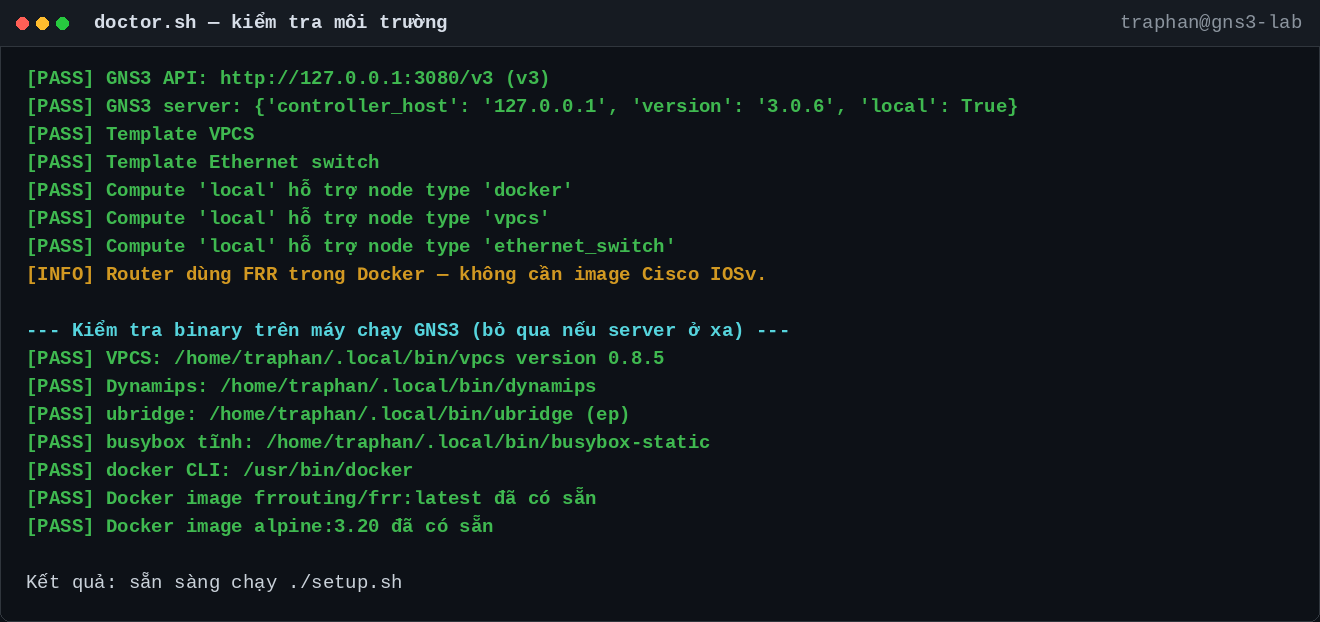
\includegraphics[width=\textwidth]{images/term-doctor.png}
  \caption{Kết quả \texttt{doctor.sh}: môi trường sẵn sàng chạy lab.}
  \label{fig:doctor}
\end{figure}

\subsection{Khởi tạo topology}

Hình~\ref{fig:setup} là kết quả \texttt{./setup.sh}. Script tạo project
\texttt{PBL3-RIPv2-DHCP-FRR}, 4 router Docker, 4 switch, 4 PC VPCS và 1 DHCP server, sau đó tạo
13 liên kết đúng với sơ đồ. Bước cuối script chờ 15 giây để RIPv2 và DHCP hội tụ rồi gọi kiểm thử
tự động.

\begin{figure}[H]
  \centering
  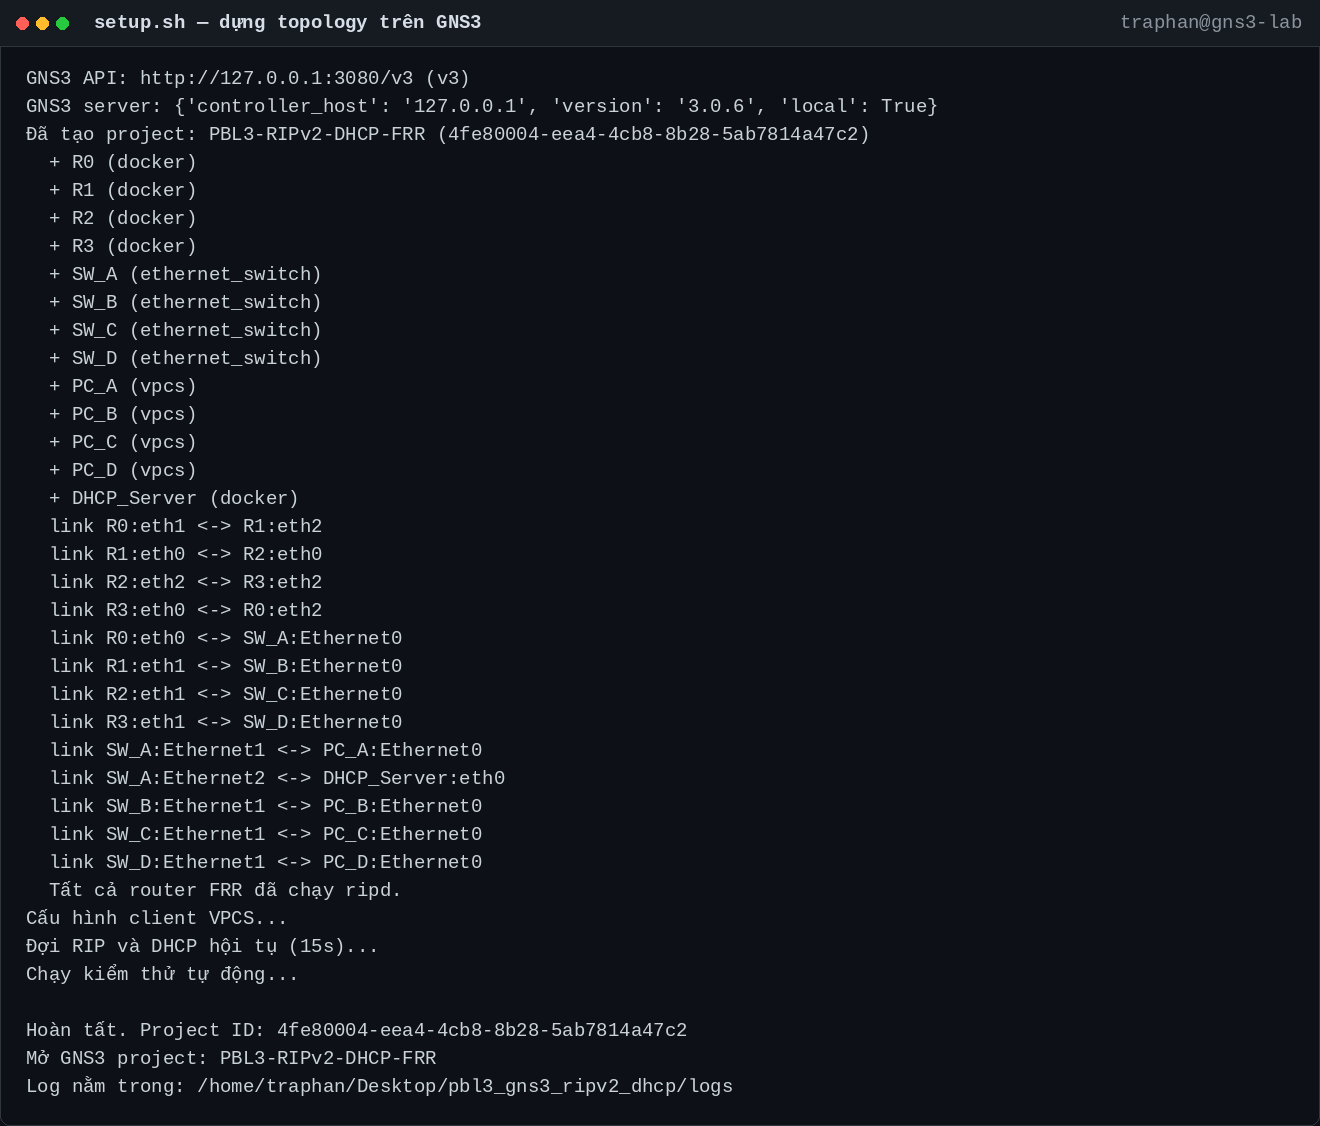
\includegraphics[width=\textwidth]{images/term-setup.png}
  \caption{Quá trình \texttt{setup.sh} tạo project, node và link.}
  \label{fig:setup}
\end{figure}

\subsection{Giao diện GNS3}

Hình~\ref{fig:gns3ui} chụp cửa sổ GNS3 đang mở project. Phía trên là thanh công cụ; bên phải là
danh sách node; phần giữa là canvas topology; phía dưới là console quản lý của GNS3. Hình~\ref{fig:gns3topo}
là ảnh cắt cận cảnh vùng topology để thấy rõ bốn router, bốn switch, bốn PC và DHCP server.

\begin{figure}[H]
  \centering
  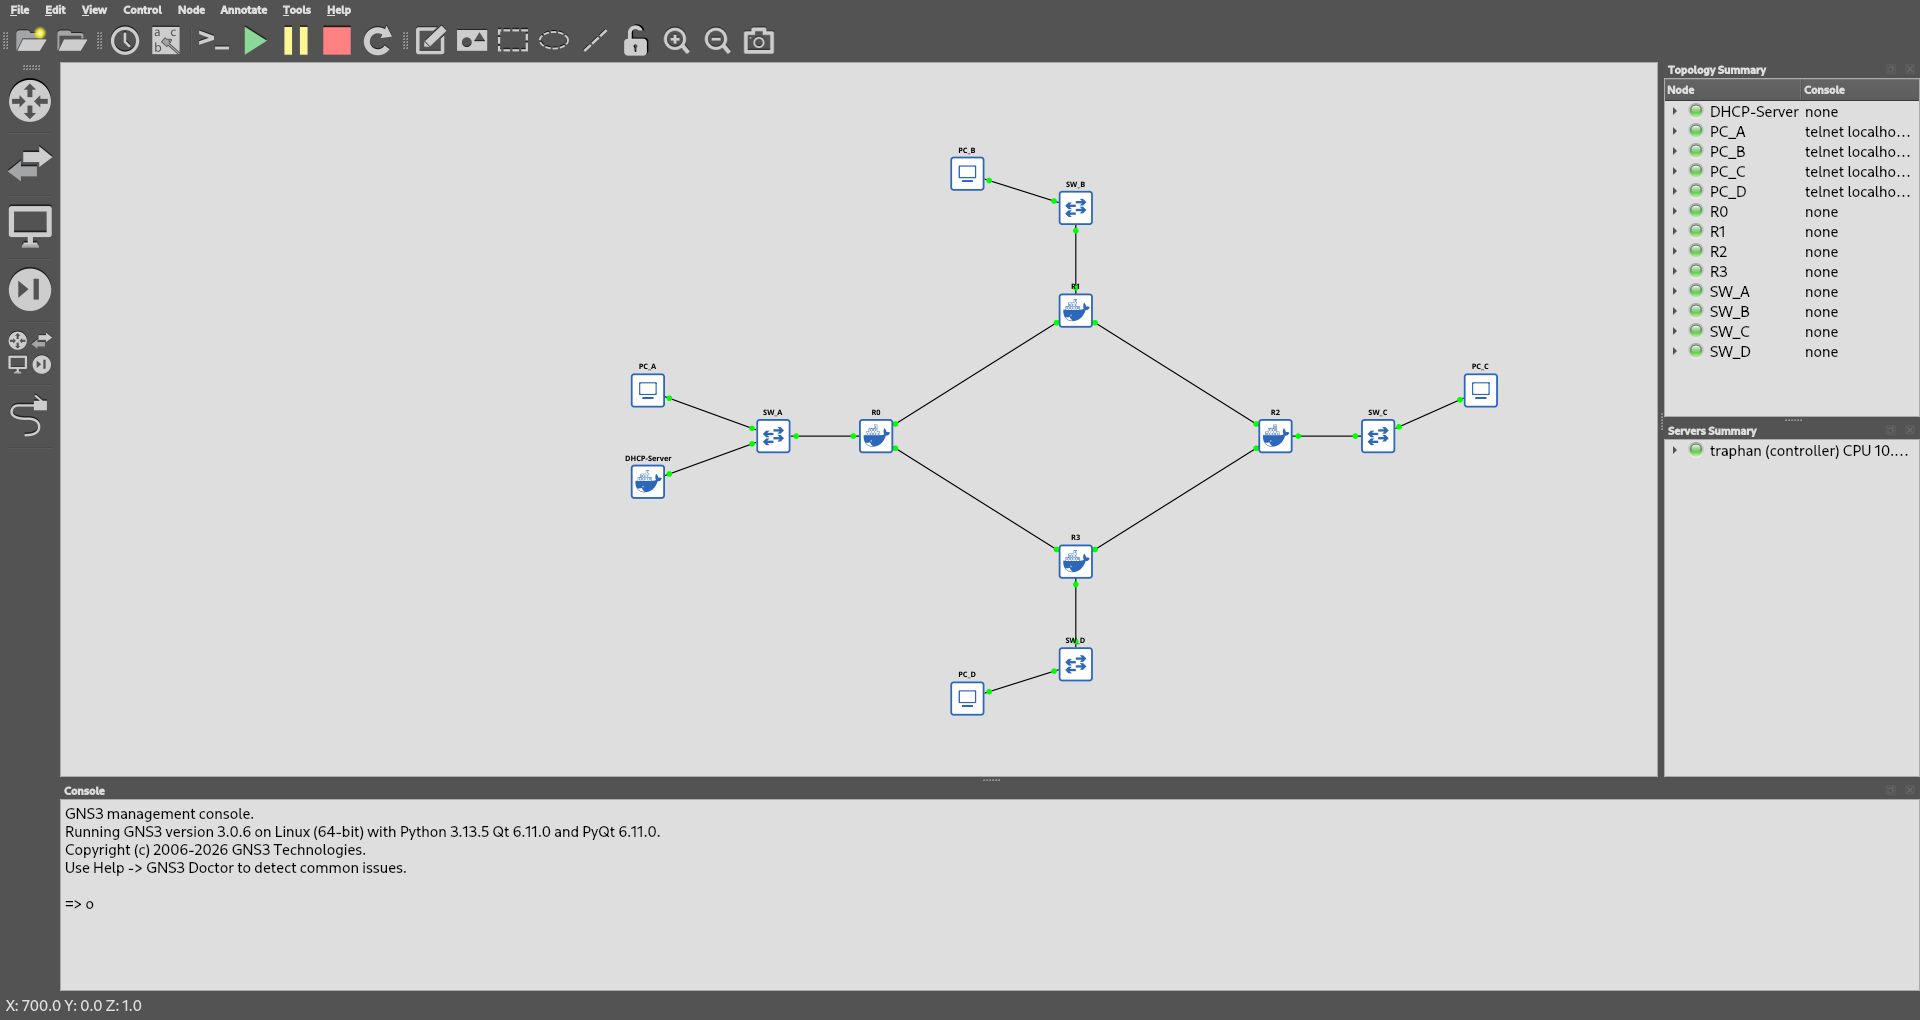
\includegraphics[width=\textwidth]{images/gns3-ui.png}
  \caption{Giao diện GNS3 3.0.6 với project \texttt{PBL3-RIPv2-DHCP-FRR}.}
  \label{fig:gns3ui}
\end{figure}

\begin{figure}[H]
  \centering
  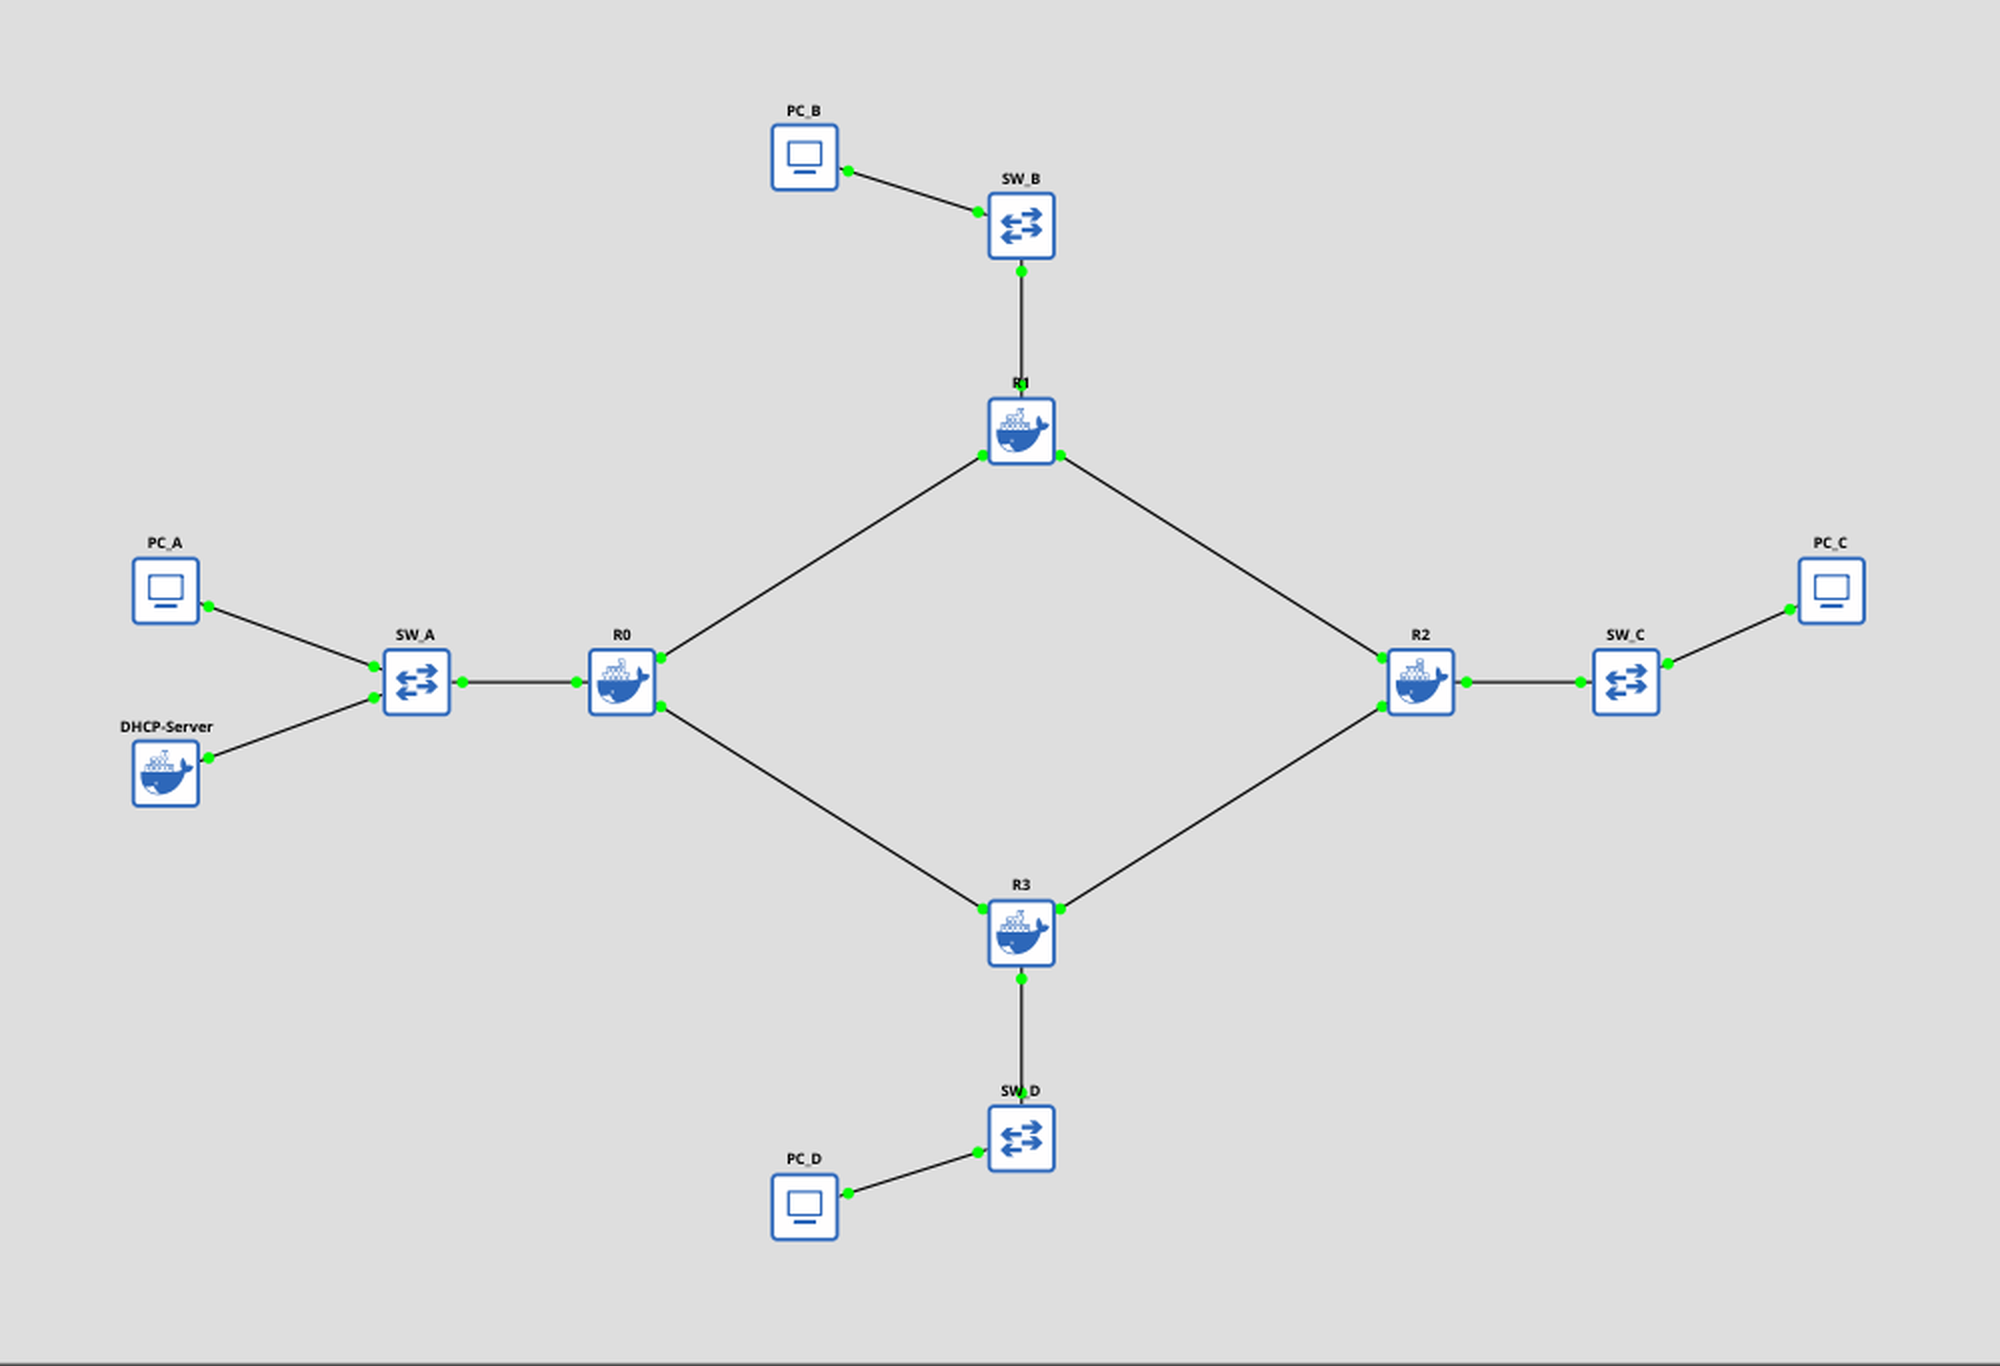
\includegraphics[width=\textwidth]{images/gns3-topology.png}
  \caption{Cận cảnh topology đang chạy trong GNS3.}
  \label{fig:gns3topo}
\end{figure}

\subsection{Container của lab}

Hình~\ref{fig:containers} liệt kê các container đang chạy. Bốn router dùng image
\texttt{frrouting/frr}, DHCP server dùng \texttt{alpine:3.20}. Tên container chứa project ID để
tránh trùng với các project GNS3 khác.

\begin{figure}[H]
  \centering
  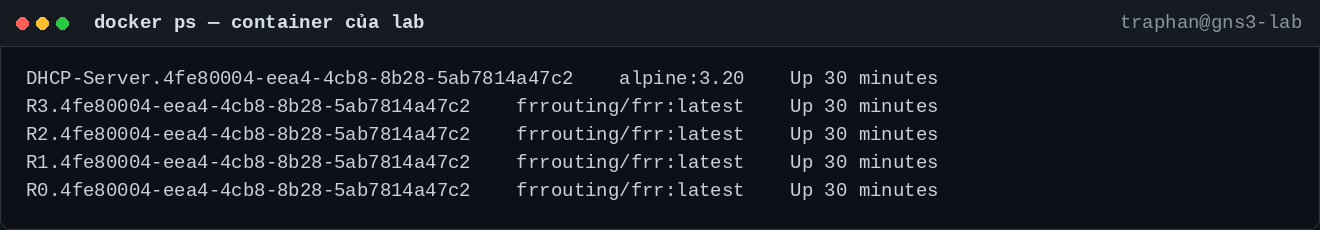
\includegraphics[width=\textwidth]{images/term-containers.png}
  \caption{Danh sách container Docker của lab.}
  \label{fig:containers}
\end{figure}

\subsection{Bảng định tuyến RIPv2}

Sau khi hội tụ, R0 có đầy đủ route trực tiếp (C) và route học qua RIP (R). Hình~\ref{fig:routes}
là kết quả \texttt{show ip route} trên R0. R0 học \texttt{10.0.23.0/24} và
\texttt{192.168.20.0/24} qua R1, học \texttt{10.0.34.0/24} và \texttt{192.168.40.0/24} qua R3;
\texttt{192.168.30.0/24} đi qua R1 với metric 3.

\begin{figure}[H]
  \centering
  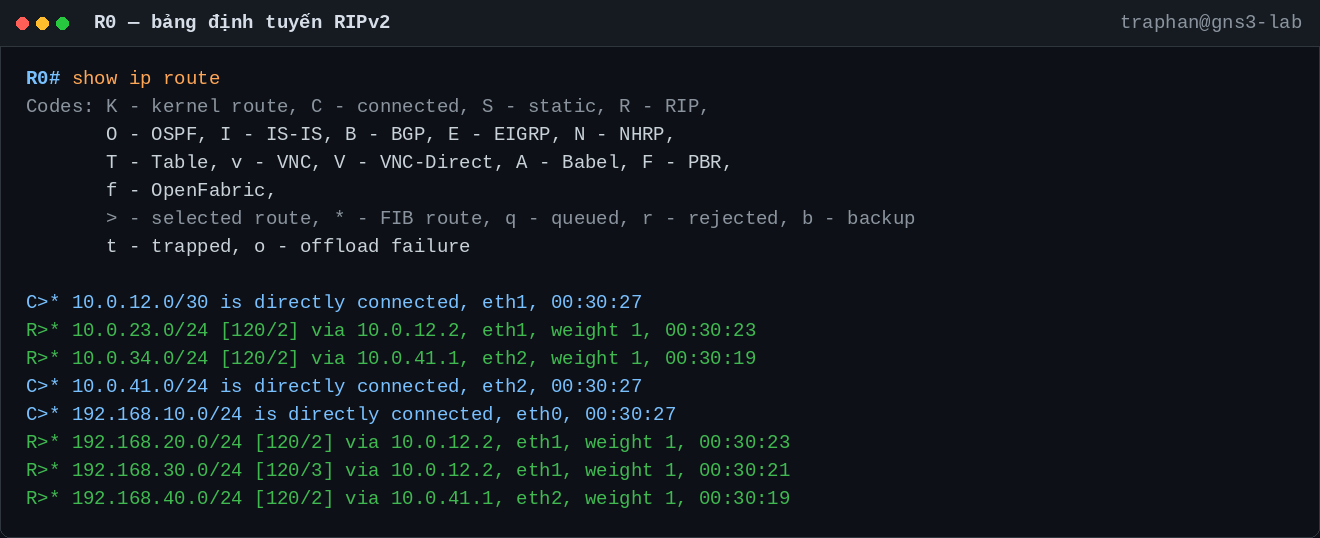
\includegraphics[width=\textwidth]{images/term-routes.png}
  \caption{Bảng định tuyến trên R0 sau khi RIPv2 hội tụ.}
  \label{fig:routes}
\end{figure}

Bảng~\ref{tab:learned} tổng hợp các route LAN học được trên cả bốn router. Ký hiệu ``C'' là kết
nối trực tiếp; ``R'' là route học qua RIP, kèm next-hop và metric.

\begin{table}[H]
  \centering
  \caption{Các mạng LAN trong bảng định tuyến của bốn router.}
  \label{tab:learned}
  \footnotesize
  \begin{tabularx}{\textwidth}{@{}l *{4}{>{\centering\arraybackslash}X}@{}}
    \toprule
    \textbf{Router} & \textbf{192.168.10.0/24} & \textbf{192.168.20.0/24} &
      \textbf{192.168.30.0/24} & \textbf{192.168.40.0/24} \\
    \midrule
    R0 & C & R, 10.0.12.2 (2) & R, 10.0.12.2 (3) & R, 10.0.41.1 (2) \\
    R1 & R, 10.0.12.1 (2) & C & R, 10.0.23.2 (2) & R, 10.0.23.2 (3) \\
    R2 & R, 10.0.23.1 (3) & R, 10.0.23.1 (2) & C & R, 10.0.34.2 (2) \\
    R3 & R, 10.0.41.2 (2) & R, 10.0.41.2 (3) & R, 10.0.34.1 (2) & C \\
    \bottomrule
  \end{tabularx}
\end{table}

\subsection{Trạng thái tiến trình RIP}

Hình~\ref{fig:rip} là kết quả \texttt{show ip rip status} trên R0. Tiến trình RIP gửi cập nhật
mỗi 30 giây, timeout 180 giây, garbage collect 120 giây, gửi/nhận version 2 trên cả ba interface.
Hai nguồn cập nhật là \texttt{10.0.12.2} (R1) và \texttt{10.0.41.1} (R3), không có bản tin lỗi
(BadPackets = 0, BadRoutes = 0), khoảng cách quản trị mặc định 120.

\begin{figure}[H]
  \centering
  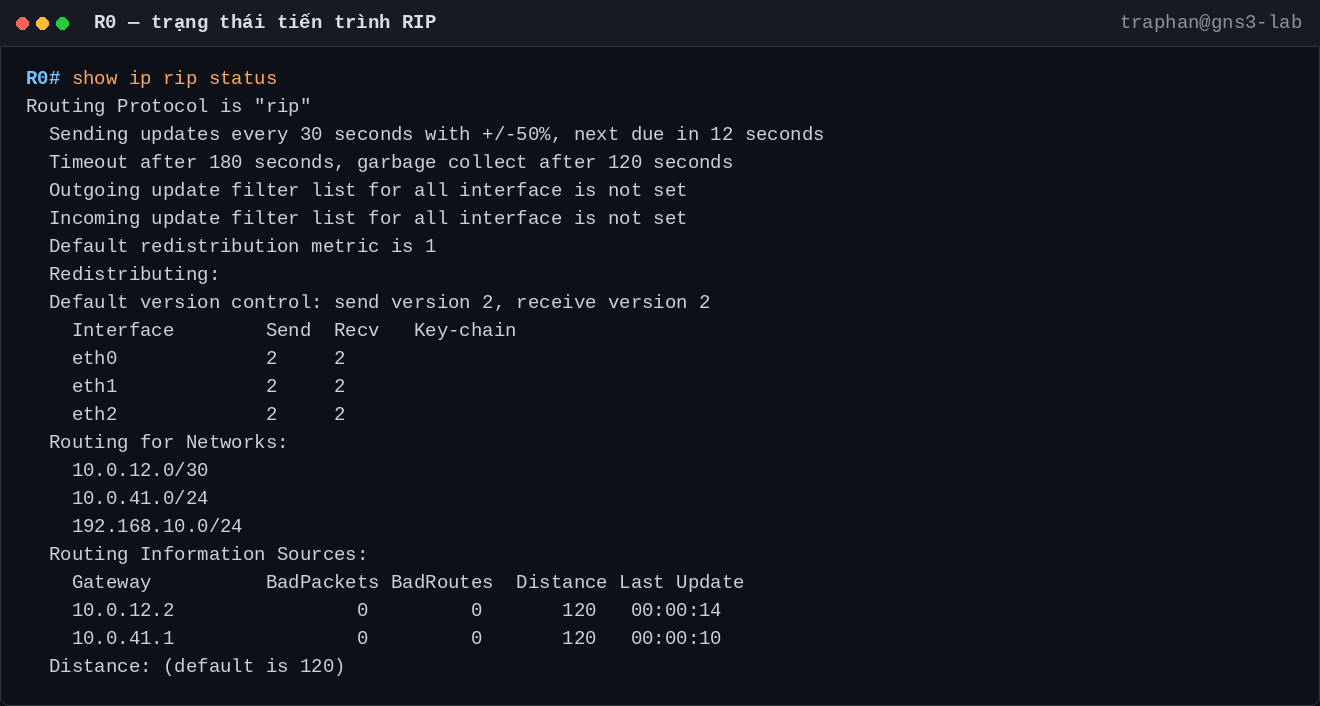
\includegraphics[width=\textwidth]{images/term-rip.png}
  \caption{Trạng thái tiến trình RIP trên R0.}
  \label{fig:rip}
\end{figure}

\subsection{Kiểm tra DHCP}

Hình~\ref{fig:dhcp} là kết quả \texttt{show ip} trên PC\_A. Máy nhận địa chỉ
\texttt{192.168.10.29/24}, gateway \texttt{192.168.10.1}, DNS \texttt{192.168.10.1} và DHCP server
\texttt{192.168.10.2}. Địa chỉ này nằm trong pool cấu hình; giá trị cụ thể có thể khác nhau giữa các lần chạy lab.

\begin{figure}[H]
  \centering
  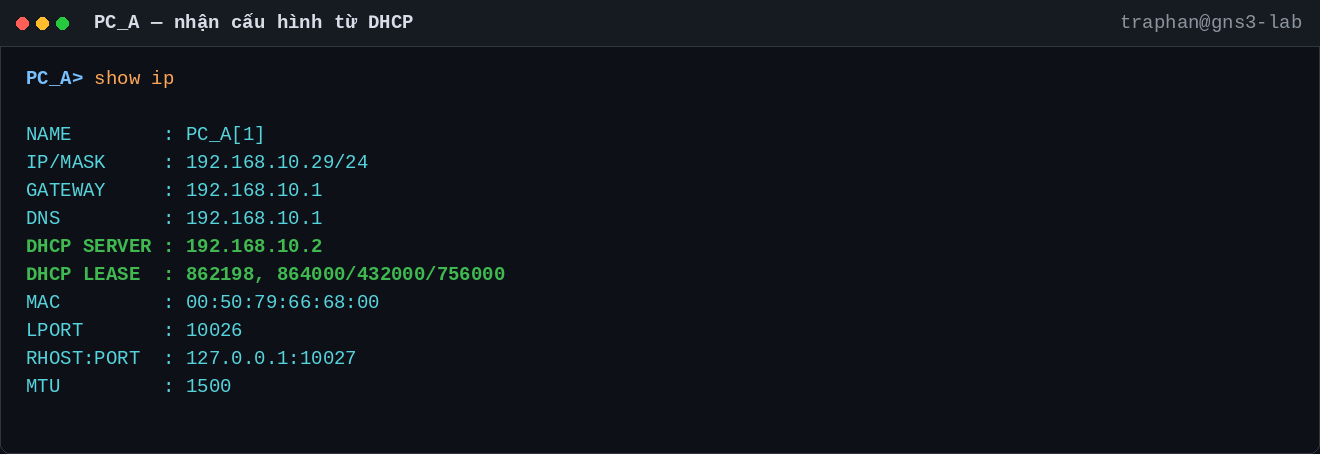
\includegraphics[width=\textwidth]{images/term-dhcp.png}
  \caption{PC\_A nhận cấu hình IP từ DHCP server.}
  \label{fig:dhcp}
\end{figure}

\subsection{Kiểm tra liên thông end-to-end}

Hình~\ref{fig:ping} minh họa một số phép ping tiêu biểu từ PC\_A và PC\_D; Bảng~\ref{tab:ping}
tổng hợp đầy đủ kết quả từ log, bao gồm cả gateway A và gateway C. Tất cả đều nhận 5/5 phản hồi.
Giá trị TTL phản ánh số hop: PC\_A tới \texttt{192.168.20.1} có TTL 63 (một router), tới
\texttt{192.168.30.1} có TTL 62 (hai router), tới \texttt{192.168.40.1} có TTL 63 (một router
theo nhánh R3).

\begin{figure}[H]
  \centering
  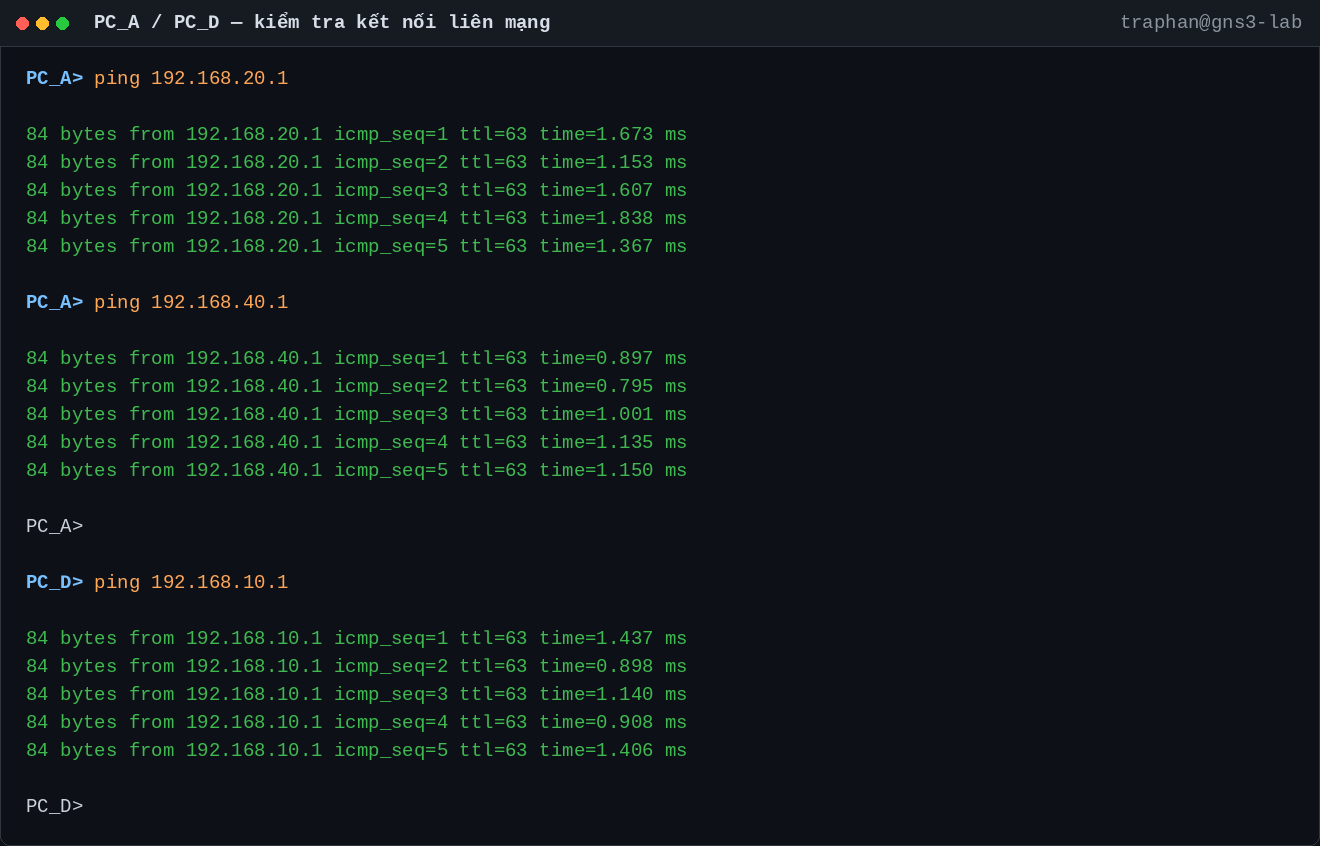
\includegraphics[width=\textwidth]{images/term-ping.png}
  \caption{Ping liên mạng từ PC\_A và PC\_D.}
  \label{fig:ping}
\end{figure}

\begin{table}[H]
  \centering
  \caption{Tổng hợp một số kết quả ping tiêu biểu.}
  \label{tab:ping}
  \begin{tabularx}{\textwidth}{@{}l l l l@{}}
    \toprule
    \textbf{Nguồn} & \textbf{Đích} & \textbf{Kết quả} & \textbf{TTL} \\
    \midrule
    PC\_A (192.168.10.29) & 192.168.10.1 (GW A) & 5/5, 100\% & 64 \\
    PC\_A (192.168.10.29) & 192.168.20.1 (GW B) & 5/5, 100\% & 63 \\
    PC\_A (192.168.10.29) & 192.168.30.1 (GW C) & 5/5, 100\% & 62 \\
    PC\_A (192.168.10.29) & 192.168.40.1 (GW D) & 5/5, 100\% & 63 \\
    PC\_D (192.168.40.10) & 192.168.10.1 (GW A) & 5/5, 100\% & 63 \\
    \bottomrule
  \end{tabularx}
\end{table}

\subsection{Kết quả kiểm thử tự động}

Hình~\ref{fig:test} là kết quả \texttt{./test.sh}. Bộ kiểm thử xác nhận bốn router có RIP và học
đủ các mạng LAN, bốn PC ping được, và PC\_A nhận địa chỉ DHCP hợp lệ. Kết quả cuối cùng là
\textbf{9/9} hạng mục PASS.

\begin{figure}[H]
  \centering
  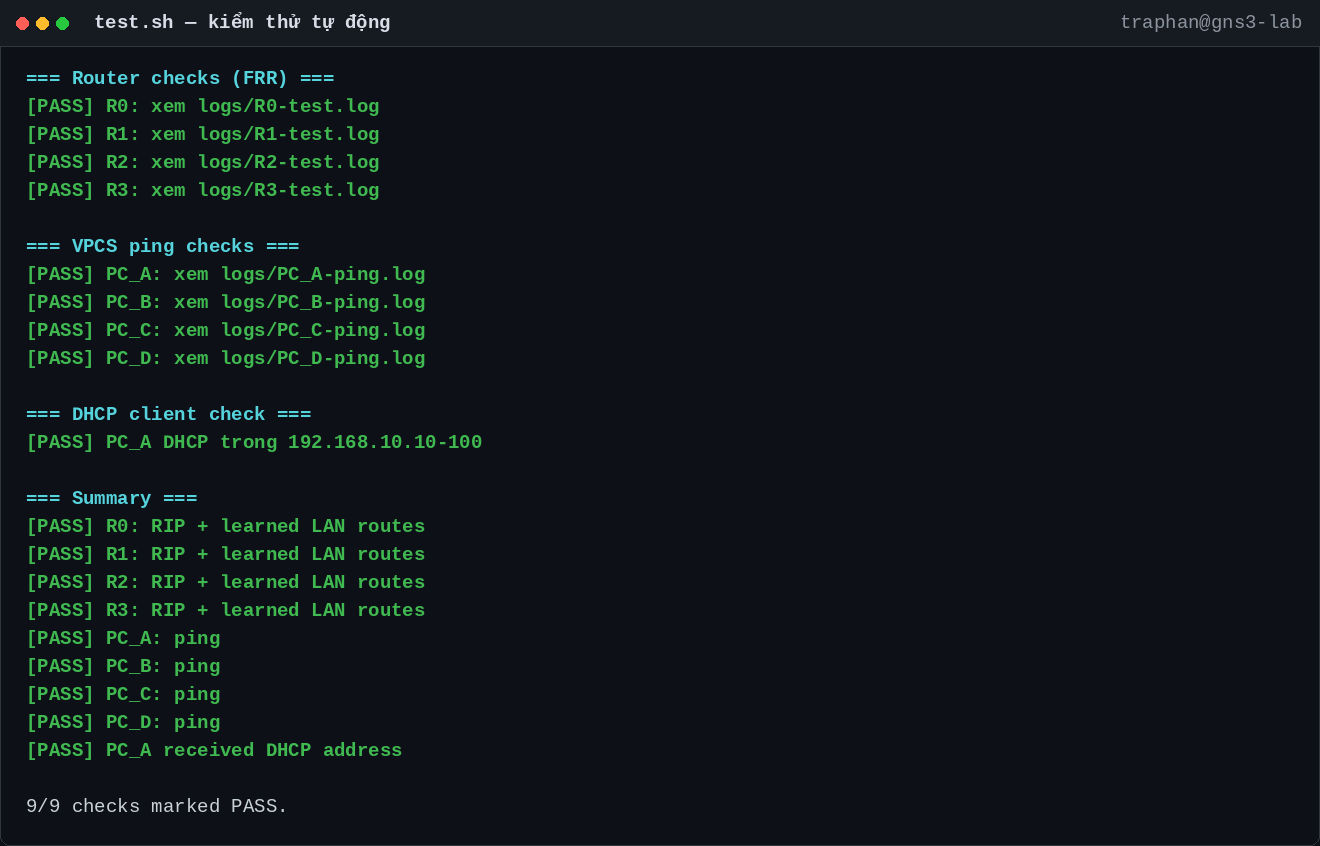
\includegraphics[width=\textwidth]{images/term-test.png}
  \caption{Kết quả \texttt{test.sh}: 9/9 kiểm thử PASS.}
  \label{fig:test}
\end{figure}

\subsection{Nhận xét về độ hội tụ và tính chịu lỗi}

Sau khoảng 15 giây, cả bốn router đã có đủ route và không còn hiện tượng mất gói trong các phép
ping. Trạng thái RIP cho thấy các bản tin cập nhật gần nhất cách thời điểm kiểm tra 10--14 giây,
phù hợp với chu kỳ 30 giây. Với topology vòng, nếu một liên kết WAN bị đứt, RIPv2 có thể học
đường thay thế qua nhánh còn lại; tuy nhiên trong phạm vi báo cáo này chưa thực hiện kịch bản
phá liên kết, nên chưa có số liệu thời gian hội tụ khi có sự cố.

% ==================================================================
\section{THẢO LUẬN}
% ==================================================================

\subsection{So sánh Packet Tracer/IOS với GNS3/FRR}

\begin{table}[H]
  \centering
  \caption{So sánh hai cách triển khai.}
  \label{tab:compare}
  \small
  \begin{tabularx}{\textwidth}{@{}l X X@{}}
    \toprule
    \textbf{Tiêu chí} & \textbf{Packet Tracer (báo cáo gốc)} & \textbf{GNS3 + FRR (báo cáo này)} \\
    \midrule
    Bản chất & Mô phỏng thiết bị và CLI Cisco & Router thật chạy FRR trong container Docker \\
    Giấy phép & Cần image IOS/IOSv có bản quyền nếu muốn IOS thật & FRR mã nguồn mở, không cần image Cisco \\
    CLI & Cisco IOS & \texttt{vtysh}, cú pháp gần IOS nhưng không giống hoàn toàn \\
    DHCP & Server0 trên GUI & Alpine + BusyBox \texttt{udhcpd} \\
    Máy trạm & Laptop mô phỏng & VPCS 0.8.5 \\
    Khả năng tái lập & Thao tác GUI, khó tự động hóa & Toàn bộ tạo bằng API/Python, có \texttt{state.json} \\
    Độ chân thực & Mô phỏng & Gần với môi trường Linux/container thật \\
    \bottomrule
  \end{tabularx}
\end{table}

\subsection{Các vấn đề gặp phải và cách xử lý}

\begin{table}[H]
  \centering
  \caption{Một số lỗi và cách khắc phục trong quá trình triển khai.}
  \label{tab:issues}
  \small
  \begin{tabularx}{\textwidth}{@{}l X X@{}}
    \toprule
    \textbf{Vấn đề} & \textbf{Nguyên nhân} & \textbf{Cách xử lý} \\
    \midrule
    Router không nhận cấu hình & API v3 yêu cầu \texttt{start\_command} nằm trong
      \texttt{properties} & Gửi \texttt{\{"properties": \{"start\_command": ...\}\}} \\
    VPCS treo khi kết nối lại & Prompt chưa được in sau khi reconnect & Gửi \texttt{\textbackslash r\textbackslash n}
      trước khi \texttt{expect(">")} \\
    Lỗi \texttt{no auto-summary} & FRR 8.4 không hỗ trợ lệnh này & Bỏ lệnh; RIPv2 mặc định classless \\
    Không có \texttt{show ip protocols} & FRR dùng lệnh khác & Dùng \texttt{show ip rip status} \\
    Thiếu image IOS & IOSv cần bản quyền & Thay bằng FRR Docker \\
    Không thấy file lease & BusyBox giữ lease trong bộ nhớ & Kiểm tra từ client bằng \texttt{show ip} \\
    \bottomrule
  \end{tabularx}
\end{table}

\subsection{Hạn chế}

\begin{itemize}[leftmargin=1.6em,itemsep=2pt]
  \item Router FRR không có console telnet trong GNS3; việc kiểm tra phải qua
        \texttt{docker exec} và \texttt{vtysh}, kém trực quan hơn console IOS.
  \item DHCP lease không được ghi ra file ổn định; khi container DHCP khởi động lại, lease cũ
        không còn. Với lab nhỏ, điều này không ảnh hưởng kết quả.
  \item Chưa kiểm thử phá liên kết WAN để đo thời gian hội tụ và kiểm chứng khả năng chịu lỗi
        của vòng.
  \item Chưa cấu hình xác thực RIPv2, route filtering, DHCP relay cho các LAN khác hoặc IPv6.
  \item Ảnh chụp GUI ở chế độ fit view có nhãn node nhỏ; sơ đồ TikZ được dùng để bổ sung phần
        trình bày trực quan.
\end{itemize}

\subsection{Bài học kinh nghiệm}

Việc chuyển một bài lab từ Packet Tracer sang GNS3 cho thấy khác biệt lớn nhất không nằm ở
topology hay địa chỉ IP, mà ở cách kiểm chứng. Với thiết bị thật, mỗi router có tiến trình riêng,
log riêng và có thể kiểm tra bằng CLI; do đó cần tự động hóa việc thu thập bằng chứng (bảng định
tuyến, trạng thái RIP, lease DHCP, ping) thay vì chỉ nhìn vào giao diện mô phỏng. Bên cạnh đó,
việc dùng API giúp tái lập lab nhanh, nhưng đòi hỏi hiểu rõ cấu trúc dữ liệu của GNS3, đặc biệt
là các trường trong \texttt{properties} của node Docker.

% ==================================================================
\section{KẾT LUẬN}
% ==================================================================

\subsection{Kết luận}

\begin{itemize}[leftmargin=1.6em,itemsep=2pt]
  \item Đã tái triển khai thành công bài lab PBL3 trên GNS3 với bốn router FRR, bốn switch, bốn
        PC và một DHCP server, giữ nguyên topology và địa chỉ IP của báo cáo gốc.
  \item RIPv2 hoạt động đúng: cả bốn router học đủ các mạng LAN, bảng định tuyến có đầy đủ route
        trực tiếp và route RIP, không có bản tin lỗi.
  \item DHCP server cấp phát thành công địa chỉ \texttt{192.168.10.29/24} cho PC\_A, kèm gateway
        và DNS đúng cấu hình.
  \item Kiểm thử end-to-end đạt 100\% cho các phép ping từ PC\_A tới bốn gateway và từ PC\_D về
        Network A; bộ kiểm thử tự động đạt 9/9.
  \item Bộ script Python và GNS3 API giúp toàn bộ quá trình tạo, kiểm tra và dọn dẹp lab có thể
        lặp lại, giảm phụ thuộc vào thao tác thủ công.
\end{itemize}

% ==================================================================
\begin{thebibliography}{9}
% ==================================================================

\bibitem{rfc2453}
G. Malkin, \emph{RIP Version 2}, RFC 2453, IETF, 1998.

\bibitem{rfc2131}
R. Droms, \emph{Dynamic Host Configuration Protocol}, RFC 2131, IETF, 1997.

\bibitem{frr}
FRRouting Project, \emph{FRRouting Documentation -- RIP}, \url{https://docs.frrouting.org/}.

\bibitem{gns3}
GNS3, \emph{GNS3 Documentation -- API v3}, \url{https://docs.gns3.com/}.

\bibitem{busybox}
BusyBox, \emph{BusyBox udhcpd}, \url{https://busybox.net/}.

\bibitem{vpcs}
GNS3, \emph{Virtual PC Simulator (VPCS)}, \url{https://github.com/GNS3/vpcs}.

\bibitem{original}
Nhóm PBL3, \emph{Báo cáo PBL3: Định tuyến động RIPv2 và máy chủ DHCP trên Cisco Packet Tracer},
2026.

\bibitem{cisco}
Cisco Systems, \emph{IP Routing: RIP Command Reference}, \url{https://www.cisco.com/}.

\end{thebibliography}

% ==================================================================
\appendix
\renewcommand{\thesubsection}{\thesection.\arabic{subsection}}
\section{CẤU HÌNH FRR ĐẦY ĐỦ}
\label{app:configs}
% ==================================================================

Phần này trình bày cấu hình của R1, R2 và R3. Cấu hình R0 đã có ở Đoạn mã~\ref{lst:r0}.

\subsection{R1}

\lstinputlisting[style=frr,caption={Cấu hình FRR của R1.}]
  {artifacts/configs/R1.conf}

\subsection{R2}

\lstinputlisting[style=frr,caption={Cấu hình FRR của R2.}]
  {artifacts/configs/R2.conf}

\subsection{R3}

\lstinputlisting[style=frr,caption={Cấu hình FRR của R3.}]
  {artifacts/configs/R3.conf}

% ==================================================================
\section{CẤU TRÚC THƯ MỤC VÀ LỆNH CHẠY}
\label{app:usage}
% ==================================================================

Cấu trúc thư mục của lab:

\begin{lstlisting}[style=plaincode,caption={Cấu trúc thư mục lab.}]
pbl3_gns3_ripv2_dhcp/
|-- setup.py                 # create project, nodes, links, config
|-- test.py                  # automated tests
|-- doctor.py                # environment checks
|-- cleanup.py               # remove project
|-- setup.sh                 # wrapper for setup.py
|-- test.sh                  # wrapper for test.py
|-- doctor.sh                # wrapper for doctor.py
|-- configs-frr/             # R0.conf ... R3.conf
|-- scripts/common.py        # shared helpers
|-- logs/                    # test logs
|-- state.json               # project id, console ports, containers
`-- report/                  # LaTeX report and images
\end{lstlisting}

Các lệnh chạy lab:

\begin{lstlisting}[style=plaincode,caption={Quy trình chạy lab.}]
./doctor.sh              # check environment
./setup.sh               # create topology and configure
# wait about 15 seconds for RIPv2 and DHCP convergence
./test.sh                # automated tests
./cleanup.sh             # remove project when done
\end{lstlisting}

Kiểm tra router FRR trực tiếp:

\begin{lstlisting}[style=plaincode,caption={Kiểm tra router qua \texttt{docker exec}.}]
docker exec GNS3.R0.<project-id> vtysh -c "show ip route"
docker exec GNS3.R0.<project-id> vtysh -c "show ip rip status"
\end{lstlisting}

% ==================================================================
\section{BẢNG KIỂM THỬ TỰ ĐỘNG}
\label{app:tests}
% ==================================================================

\begin{table}[H]
  \centering
  \caption{Danh sách 9 hạng mục kiểm thử.}
  \label{tab:testmatrix}
  \begin{tabularx}{\textwidth}{@{}c l X c@{}}
    \toprule
    \textbf{STT} & \textbf{Hạng mục} & \textbf{Nội dung kiểm tra} & \textbf{Kết quả} \\
    \midrule
    1 & R0 & Có tiến trình RIP và đủ route LAN 20/30/40 & PASS \\
    2 & R1 & Có tiến trình RIP và đủ route LAN 10/30/40 & PASS \\
    3 & R2 & Có tiến trình RIP và đủ route LAN 10/20/40 & PASS \\
    4 & R3 & Có tiến trình RIP và đủ route LAN 10/20/30 & PASS \\
    5 & PC\_A & Ping được bốn gateway & PASS \\
    6 & PC\_B & Ping được gateway B và A & PASS \\
    7 & PC\_C & Ping được gateway C và A & PASS \\
    8 & PC\_D & Ping được gateway D và A & PASS \\
    9 & DHCP & PC\_A nhận IP trong dải 192.168.10.10--100 & PASS \\
    \bottomrule
  \end{tabularx}
\end{table}

\end{document}
